\documentclass[fleqn]{homework}

\student{Stephen Brennan (smb196)}
\course{EECS 440}
\assignment{Programming 4}
\duedate{November 19, 2015}

%\usepackage{mathtools}
%\usepackage{graphicx}
\usepackage{booktabs}
\usepackage{placeins}

\begin{document}
  \maketitle

  \section{Implementation Commentary}

  For the most part, implementing bagging and boosting was rather simple.  My
  original implementation of decision trees had to be slightly optimized in
  order to provide reasonable performance in this situation.  In particular, my
  selection of a cutoff for continuous variables was inefficient originally: it
  recomputed mutual information (an linear time operation in the number of
  examples) for every potential cutoff (which is also linear in the number of
  examples).  This gave an overall quadratic runtime.  I was able to improve
  this by doing a single iteration over the sorted values for the continuous
  feature.  For each variable, I updated counts (more accurately, weights) of
  examples on either side of the split, and incrementally recomputed the mutual
  information, resulting in a linear time operation.  Accounting for the time to
  sort the examples by their attribute value, this resulted in an $O(n \log n)$
  improvement, which was very noticeable.

  Implementing weights for decision trees was simple.  Most of the modifications
  were the mutual information procedure (using weights instead of counts for
  computing probabilities).  The other critical change was to select the
  majority class label (at leaves) based on the total weights, not on the
  counts.  When I did this, Boosting started giving better results.

  Implementing weights for neural networks was also rather simple.  Instead of
  using the squared loss function $L(\hat{y_i}, y_i) = (\hat{y}_i - y_i)^2$, I
  used a weighted squared loss function:
  $L(\hat{y_i}, y_i) = w_i (\hat{y}_i - y_i)^2$.  Thus, the weights were simply
  multiplied into the gradient for each example.

  Also, it is worth noting that my implementations and changes only went so far
  as the assignment description specified.  That is, I have not tested and will
  not certify that these work when the parameters (for instance, decision tree
  depth or neural net layers) are set to values not specified from the
  assignment description.  So, when using my code, please use the following
  arguments:

  \begin{itemize}
  \item For decision trees, be sure to set \texttt{--depth} to 2 (this means
    level of decision nodes, and then leaf nodes).
  \item For neural networks, be sure to set \texttt{--layer\_sizes} to 0 (no
    hidden layer) and \texttt{--max\_iters} to something reasonable (I used 5000
    in all my tests), since convergence never seems to be a guarantee in my
    neural network implementation.
  \end{itemize}

  \begin{problem}{a}
    \begin{question}
      For all problems and the two learning algorithms, compare the accuracy of
      the ensemble versions (10 iterations) to the base learners. Produce a
      table with the accuracies of the base learner, the bagged learner, and the
      boosted learner. Perform paired $t$-tests to determine if any of the
      ensemble methods are significantly better than the base learner with 95\%
      confidence.
    \end{question}
    \FloatBarrier

    \begin{table}[h]
    \centering
    \caption{Comparison of base, bagged, and boosted learners.}
    \label{t:a-comparison}
    \begin{tabular}{llll|lll}
      \toprule
      Problem & \multicolumn{3}{c}{Decision Tree} & \multicolumn{3}{c}{Neural Network} \\
      \midrule
             & Base          & Bagging       & Boosting      & Base          & Bagging      & Boosting       \\
      Voting & 0.989 (0.007) & 0.982 (0.015) & 0.984 (0.012) & 0.984 (0.012) & 0.986 (0.009) & 0.977 (0.012) \\
      Spam   & 0.711 (0.002) & 0.710 (0.002) & 0.717 (0.005) & 0.647 (0.034) & 0.657 (0.035) & 0.697 (0.003) \\
      Volcanoes&0.672 (0.001)& 0.672 (0.001) & 0.773 (0.018) & 0.833 (0.028) & 0.839 (0.014) & 0.820 (0.023) \\
      \bottomrule
    \end{tabular}
    \end{table}

    A comparison of the accuracies is presented in Table~\ref{t:a-comparison}.
    Numbers in parentheses are (uncorrected) standard deviations.  Resulting
    95\% confidence intervals are presented in Table~\ref{t:a-ci}

    \begin{table}[h]
      \centering
      \caption{Confidence intervals for difference of ensemble and base learner means.}
      \label{t:a-ci}
      \begin{tabular}{lcccc}
        \toprule
        Problem   & \multicolumn{2}{c}{Decision Tree} & \multicolumn{2}{c}{Neural Network} \\
        \midrule
                  & Bagging         & Boosting        & Bagging         & Boosting \\
        Voting    & (-0.012, 0.026) & (-0.011, 0.021) & (-0.019, 0.015) & (-0.013, 0.027)\\
        Spam      & (-0.005, 0.007) & (-0.014, 0.002) & (-0.066, 0.046) & (-0.089, -0.011)\\
        Volcanoes & (-0.002, 0.002) & (-0.122, -0.080)& (-0.042, 0.030) & (-0.029, 0.055)\\
        \bottomrule
      \end{tabular}
    \end{table}

    According to the confidence intervals in Table~\ref{t:a-ci}, Boosting
    improved the Decision Tree's performance on Volcanoes significantly, and the
    Neural Network's performance on Spam significantly.
  \end{problem}

  \begin{problem}{b}
    \begin{question}
      For any two problems and the two learning algorithms, evaluate how the
      accuracy of bagging changes with the number of iterations. Pick at least
      three iteration values between 2 and 50, and plot the accuracy on a
      graph. Do you see any difference by problem? By algorithm?
    \end{question}

    \begin{table}[h]
      \centering
      \caption{Effect of iterations of bagging on accuracy.}
      \label{t:b}
      \begin{tabular}{ll|ll}
        \toprule
        Problem   & Iterations & Decision Tree Accuracy & Neural Network Accuracy \\
        \midrule
                  & 2          & 0.984 (0.014)          & 0.982 (0.012)            \\
        Voting    & 35         & 0.989 (0.010)          & 0.986 (0.009)            \\
                  & 50         & 0.984 (0.015)          & 0.984 (0.012)            \\
        \midrule
                  & 2          & 0.676 (0.007)          & 0.827 (0.015)            \\
        Volcanoes & 35         & 0.672 (0.001)          & 0.848 (0.014)            \\
                  & 50         & 0.672 (0.001)          & 0.845 (0.027)            \\
        \bottomrule
      \end{tabular}
    \end{table}

    These findings are presented in Figures~\ref{f:b-voting} and
    ~\ref{f:b-volcanoes}.  Please note the $y$ scales on these plots.

    \begin{figure}[h!]
      \centering
      \caption{}
      \label{f:b-voting}
      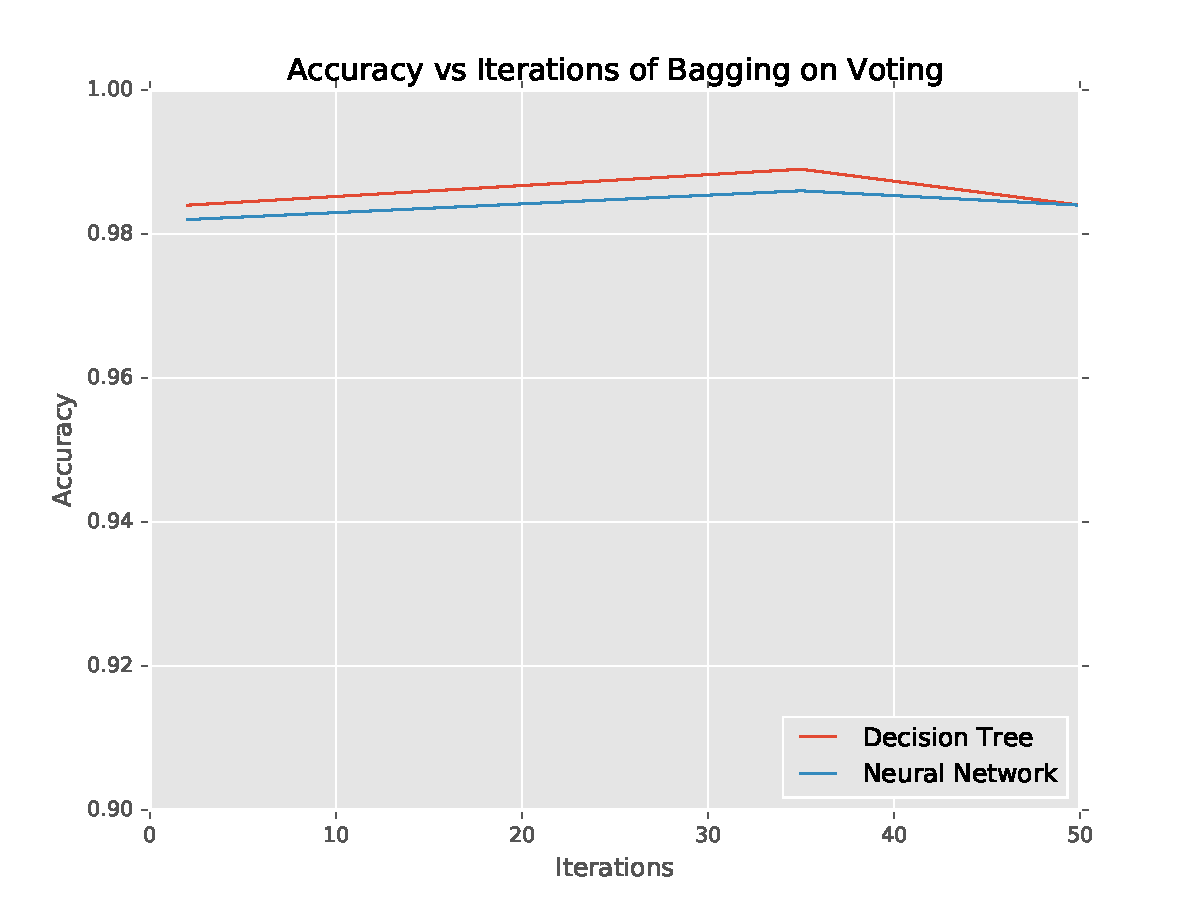
\includegraphics[width=0.67\textwidth]{b-voting.pdf}
    \end{figure}
    \begin{figure}[h!]
      \centering
      \caption{}
      \label{f:b-volcanoes}
      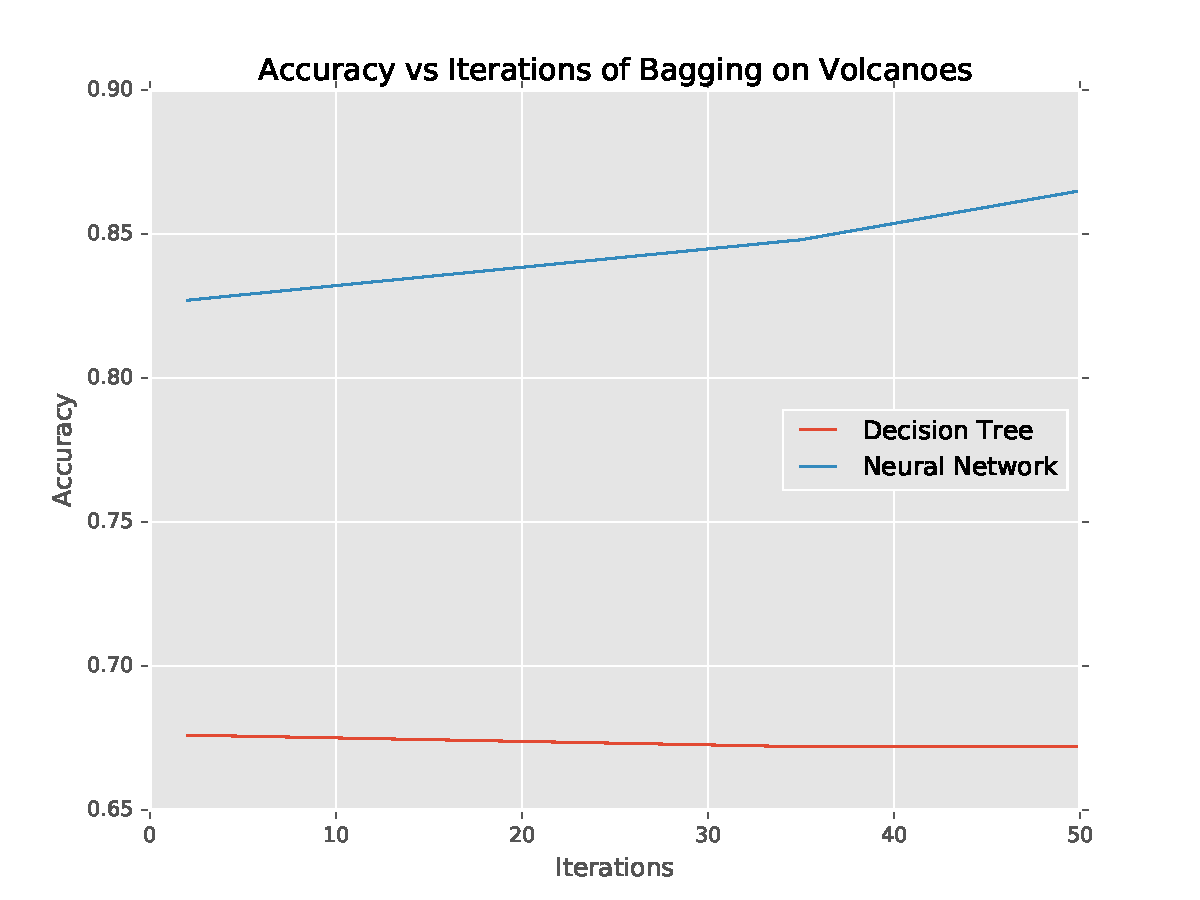
\includegraphics[width=0.67\textwidth]{b-volcanoes.pdf}
    \end{figure}

    Overall, it seems that bagging did not help with voting very much, probably
    because it already had very good accuracy.  Bagging showed mild improvement
    for the neural network, but not for the decision tree.  I noticed that
    bagging became a majority class label predictor for decision tree on
    volcanoes, when you set the iterations high.  I wonder if this is due to the
    fact that decision trees are in general a rather poor predictor for large
    amounts of continuous attributes like volcanoes.
  \end{problem}

  \begin{problem}{c}
    \begin{question}
      Repeat (b) for boosting.
    \end{question}
  \end{problem}

  \begin{problem}{d}
    \begin{question}
      Evaluate the sensitivity of bagging to noise as follows. When training,
      after constructing the training sample, flip an example’s label with
      probability $p$. Then use this noisy sample in your bagging algorithm and
      evaluate the resulting classifier on the usual (noise free) test set. For
      any two problems and any two learning algorithms, plot a graph with $p$ on
      the $x$-axis and the test-set accuracy of bagging (30 iterations) on the
      $y$-axis. You can use results from the previous questions for a $p=0$
      point. Discuss how resilient bagging is to noise based on your
      observations.
    \end{question}
  \end{problem}

  \begin{problem}{e}
    \begin{question}
      Repeat (d) for boosting.
    \end{question}
  \end{problem}

\end{document}